\begin{figure*}[t]
  \centering
  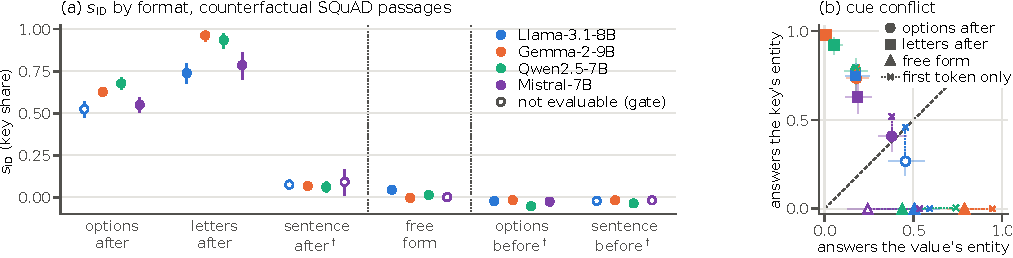
\includegraphics[width=\textwidth]{figures/fig_natural.pdf}
  \caption{\textbf{On passages, a later options list makes the model read the answer entity's identity through its cached keys; with lettered options, generated answers follow the key's entity in all four models.} Counterfactual SQuAD passages, four models, 185 items; 95\,\% two-stage article-cluster intervals. (a)~$s_{\mathrm{ID}}$ by format, at the first answer token; hollow: failed a preregistered quality gate; $\dagger$: recomputed (exploratory). (b)~Cue conflict (key and value from two counterfactual entities): answers naming the key's or the value's entity; crosses: decision token alone; a boundary, not a confirmed claim.}
  \label{fig:natural}
\end{figure*}

\section{Later mentions decide whether a value is looked up or copied}\label{sec:claim1}

\textbf{When the candidates are listed again after the writing token, later tokens read its key, which carries most of the value's identity (a sentence naming them opens part of that read); without a later mention the identity is copied from the value.} Position decides, and the decision reaches generated answers. We call this the \emph{format law}.

\subsection{Fresh stories in seven families}\label{sec:fresh}

In the discovery sample (\cref{app:discovery}) a list after the story opened a large key read, also on two further tasks, an instruction-matched $2{\times}2$ showed that position decides, and the channels carried which value was written, not its belief role.\label{sec:scope} The confirmation ran on the 150 fresh stories in four discovery-sample models (Qwen2.5-7B and 14B, Mistral-7B, OLMo-2-7B) and four families never examined before (\cref{fig:schematic}b). With the candidates listed after the story, the writing token's key carries most of the value's identity in all eight models, the new families included ($s_{\mathrm{ID}}$ = \JbRangeSidAfterEightMin--\JbRangeSidAfterEightMax). Without a later mention, the identity is copied through the value in every family ($s_{\mathrm{ID}}$ = $\JbRangeSidNoneEightMin$ to \JbRangeSidNoneEightMax). The same list or sentence before the story opens no key read ($s_{\mathrm{ID}}$ = $\JbRangeSidBeforeEightMin$ to $\JbRangeSidBeforeEightMax$ with the list before); in the four new families the read with a list before is even below its no-mention level ($r$ = $\JbRangeRBeforeNfourMin$ to $\JbRangeRBeforeNfourMax$, against \JbRangeRNoneNfourMin--\JbRangeRNoneNfourMax{} without a mention), which we do not explain (\cref{sec:limitations}).

A neutral sentence naming the candidates after the story opens an intermediate key read, $r$ = \JbRangeRPostEightMin--\JbRangeRPostEightMax{} of the list read over the eight models. A sentence of the same length naming no candidate opens at most a negligible read beyond the no-mention level ($r \leq \JbRangeRPostNullEightMax$; at Llama-3.1-8B, $+0.005$ [0.0001, 0.011] over no mention, a 98.75\,\% interval, post hoc), so the read needs the re-mention. Gemma-2-2B failed the competence gate (accuracy \JbGfiveAccPostGemmaTwo{} with the sentence, against 0.8), so its test could not be evaluated; read post hoc, its sentence read is small but not absent, $r$ = \ci{\JbRPostGemmaTwo}{\JbRPostGemmaTwoLo}{\JbRPostGemmaTwoHi} (\cref{app:fresh}). % verbatim: "+0.005 [0.0001, 0.011]", outcome J part B

\paragraph{Generated answers.}
Clamping only the key changes the generated answer to the clamped value in \pctn{\JbRangeBetaKAfterEightMin}--\pct{\JbRangeBetaKAfterEightMax} of stories when the candidates are listed after the story and in at most \pct{\JbRangeBetaKNoneEightMax} when they are not; clamping only the value does the reverse (\cref{fig:schematic}c). (`Not': no mention, a list or a sentence before; without a mention the value-only clamp changes \pctn{\JbRangeBetaVNoneEightMin}--\pct{\JbRangeBetaVNoneEightMax}.) The sentence read changes generated answers in seven of the eight models (flip rate \pctn{\JbFivebFlipPostMetMin}--\pct{\JbFivebFlipPostMetMax} after the sentence, \pct{\JbRangeFlipPreEightMax} before it), a small share in most; at OLMo-2-7B the read is visible in log-probabilities but hardly in generated answers (flip rate 1.0\,\% after, 0\,\% before). % verbatim: outcome J part B

\paragraph{The measurement.}
Scored on the emitted forms (coverage $\geq 0.8$ in every cell), every re-scored discovery-sample result is unchanged, and $s_{\mathrm{ID}}$ moves by at most 0.05; but the sentence read relative to the list read, $r$, rises by $+$\ci{\JbSixbRPostMistralSeven}{\JbSixbRPostMistralSevenLo}{\JbSixbRPostMistralSevenHi} at Mistral-7B and $+$\ci{\JbSixbRPostQwenFourteen}{\JbSixbRPostQwenFourteenLo}{\JbSixbRPostQwenFourteenHi} at Qwen2.5-14B: the lower-case score understated the sentence read (two further validity checks: \cref{app:measure}).

\subsection{Reading-comprehension passages}\label{sec:natural}

On counterfactual SQuAD passages, a later options list makes the model read the passage entity through its cached keys ($s_{\mathrm{ID}}$ \JaSidOptaMistralSeven--\JaSidOptaQwenSeven{} in Gemma-2-9B, Qwen2.5-7B and Mistral-7B, \JaOnebSidMistralSeven--\JaOnebSidQwenSeven{} for answers of three or more tokens, and \JaSidLetaLlamaEight--\JaSidLetaGemmaNine{} with lettered options in all four models), and without it through its values ($s_{\mathrm{ID}}$ at most \JaSidNomLlamaEight{} in Llama-3.1-8B, Gemma-2-9B and Qwen2.5-7B; \cref{fig:natural}a). Options before the passage leave a small negative key read. A related-articles sentence after the passage opens only a small key read ($s_{\mathrm{ID}}$ gain \ci{\JaFiveDiffQwenSeven}{\JaFiveDiffQwenSevenLo}{\JaFiveDiffQwenSevenHi} at Qwen2.5-7B and \ci{\JaFiveDiffGemmaNine}{\JaFiveDiffGemmaNineLo}{\JaFiveDiffGemmaNineHi} at Gemma-2-9B), so on passages our claim concerns a later options list. Of the 24 model--format cells, \JaGateFailCells{} failed a preregistered quality gate and enter no comparison (\cref{app:natural}), among them Llama-3.1-8B's options-after and Mistral-7B's free-form cells; the within-model difference between options after and free form could therefore be evaluated only at Gemma-2-9B and Qwen2.5-7B (\JaThreeDiffGemmaNine{} and \JaThreeDiffQwenSeven), and under one of two conflicting rules the gate failures would have restricted the title to templated stories (\cref{app:decisions}).

\paragraph{Behaviour on passages is a boundary.}
In cue conflict (key and value from two counterfactual entities), with lettered options the generated answer follows the key's entity in all four models (key-source rate \JaKeySrcLetaMistralSeven--\JaKeySrcLetaGemmaNine; lowest at Mistral-7B, \ci{\JaKeySrcLetaMistralSeven}{\JaKeySrcLetaMistralSevenLo}{\JaKeySrcLetaMistralSevenHi}). With options answered by name the key's entity is named in most answers at Gemma and Qwen (\JaKeySrcOptaGemmaNine{} and \JaKeySrcOptaQwenSeven) but at Mistral in \ci{\JaKeySrcOptaMistralSeven}{\JaKeySrcOptaMistralSevenLo}{\JaKeySrcOptaMistralSevenHi}, about as often as the value's (\JaValSrcOptaMistralSeven), and a key that matches no option leaves the value to be copied. In free form the decision token follows the value while the continuation breaks (hybrids, an observation), so few whole answers name the value's entity (\cref{fig:natural}b). The channel attributions are therefore not shown to decide behaviour on natural text. In the one model with enough items, Qwen2.5-7B, 2-bit quantization of values against keys shows no clear format difference (\ci{$\JaSevenDiDQwenSeven$}{$\JaSevenDiDQwenSevenLo$}{\JaSevenDiDQwenSevenHi}), a key matching no candidate leaves hybrids in \ci{\JaEightdNomGemmaNine}{\JaEightdNomGemmaNineLo}{\JaEightdNomGemmaNineHi} of free-form answers (Gemma-2-9B), and the reader heads' passage tests (\cref{sec:claim2}) and three others failed their gates (\cref{app:natural}).
